\documentclass[tikz,border=8pt]{standalone}
% Shared look for every TikZ diagram. Load with \input{../../tools/tikz-style.tex}
\usepackage[T1]{fontenc}
\usepackage{lmodern}
\renewcommand{\sfdefault}{lmr}  % diagrams use the same serif as the text
\usetikzlibrary{arrows.meta, positioning, shapes.geometric, calc, fit, backgrounds}
\definecolor{cblue}{HTML}{4C78A8}
\definecolor{corange}{HTML}{F58518}
\definecolor{cgreen}{HTML}{54A24B}
\definecolor{cred}{HTML}{E45756}
\definecolor{cpurple}{HTML}{B279A2}
\definecolor{cgrey}{HTML}{6B6B6B}
\tikzset{
  every picture/.style={font=\sffamily, line width=1.2pt},
  box/.style={draw=#1, fill=#1!12, rounded corners=4pt, align=center, inner sep=7pt, minimum height=1.1cm},
  box/.default=cgrey,
  arrow/.style={-{Stealth[length=3mm]}, draw=cgrey, line width=1.4pt},
  title/.style={font=\sffamily\bfseries\Large},
  note/.style={font=\sffamily\small, text=cgrey, align=center},
}
\AtBeginDocument{\hyphenpenalty=10000 \exhyphenpenalty=10000}

\usetikzlibrary{shadings}
\begin{document}
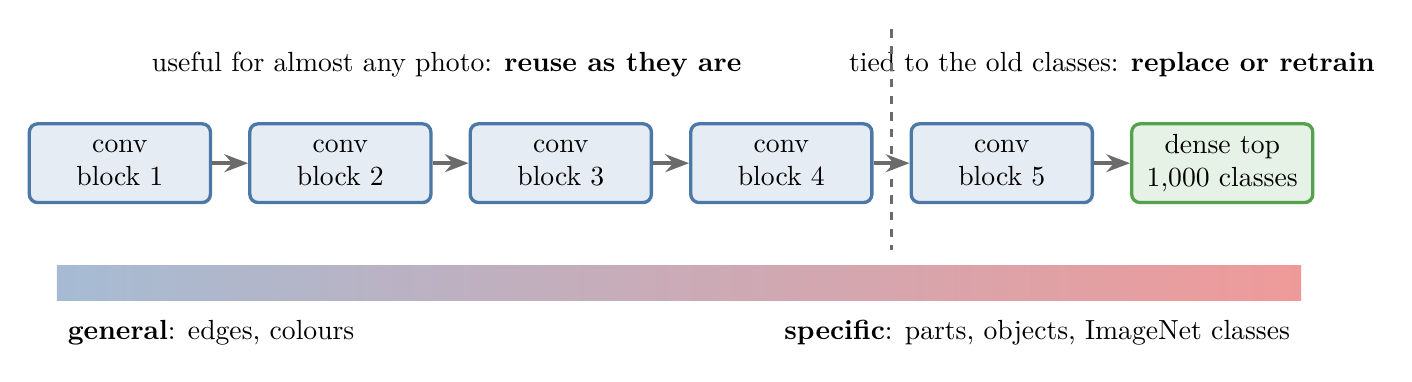
\begin{tikzpicture}[blk/.style={draw=cblue, fill=cblue!14, rounded corners=3pt, minimum width=2.3cm, minimum height=1.0cm, font=\sffamily\normalsize, align=center}]
  \foreach \k in {1,...,5} \node[blk] (b\k) at (2.8*\k,0) {conv\\block \k};
  \node[blk, draw=cgreen, fill=cgreen!14] (top) at (16.8,0) {dense top\\1,000 classes};
  \foreach \a/\b in {b1/b2,b2/b3,b3/b4,b4/b5,b5/top} \draw[arrow] (\a) -- (\b);
  \shade[left color=cblue!50, right color=cred!60] (2.0,-1.3) rectangle (17.8,-1.75);
  \node[anchor=west, font=\sffamily\normalsize] at (2.0,-2.15) {\textbf{general}: edges, colours};
  \node[anchor=east, font=\sffamily\normalsize] at (17.8,-2.15) {\textbf{specific}: parts, objects, ImageNet classes};
  \node[font=\sffamily\normalsize, align=center] at (6.95,1.25) {useful for almost any photo: \textbf{reuse as they are}};
  \node[font=\sffamily\normalsize, align=center] at (15.4,1.25) {tied to the old classes: \textbf{replace or retrain}};
  \draw[cgrey, dashed] (12.6,1.7) -- (12.6,-1.1);
\end{tikzpicture}
\end{document}
